\documentclass{article}
\usepackage[UTF8]{ctex}
\usepackage[T1]{fontenc}
\usepackage[utf8]{inputenc}
\usepackage{titlesec}
\usepackage{xcolor}
\usepackage{tikz}
\usepackage{subfigure}
\usetikzlibrary{positioning}
\usetikzlibrary[arrows, shapes, chains]

\titleformat{\section}[block]{\LARGE\scshape}{\arabic{section}}{1em}{}[]

\tikzset{
    normal/.style = {ellipse, draw = black, text ragged, minimum width = 6em, scale = 0.35},
    expand/.style = {ellipse, draw = red!70!black, text ragged, minimum width = 6em, black, fill = red!30!white, scale = 0.35},
    length/.style = {text ragged, scale = 0.25},
    level distance = 5em,
    level 1/.style = {sibling distance = 60em},
    level 2/.style = {sibling distance = 30em},
    level 3/.style = {sibling distance = 20em},
    level 4/.style = {sibling distance = 8em},
    level 5/.style = {sibling distance = 10em},
}

\title{Homework 2}
\author{PB17000297 罗晏宸}
\date{March 8 2020}

\begin{document}
\maketitle

\section{Exercise 3.6}
跟踪A$^*$算法应用直线距离启发式求解从 Lugoj 到 Bucharest 问题的过程。给出结点扩展的顺序和每个结点的$f$、$g$ 和 $h$ 值。

\paragraph{解}
Romania 问题中到 Bucharest 的直线距离如表所示:
\begin{table}[h]
    \centering
    \begin{tabular}{lrlr}
    \textbf{Arad}      & 366 & \textbf{Mehadia}        & 241 \\
    \textbf{Bucharest} & 0   & \textbf{Neamt}          & 234 \\
    \textbf{Craiova}   & 160 & \textbf{Oradea}         & 380 \\
    \textbf{Drobeta}   & 242 & \textbf{Pitesti}        & 100 \\
    \textbf{Eforie}    & 161 & \textbf{Rimnicu Vilcea} & 193 \\
    \textbf{Fagaras}   & 176 & \textbf{Sibiu}          & 253 \\
    \textbf{Giurgiu}   & 77  & \textbf{Timisoara}      & 329 \\
    \textbf{Hirsova}   & 151 & \textbf{Urziceni}       & 80  \\
    \textbf{Iasi}      & 226 & \textbf{Vaslui}         & 199 \\
    \textbf{Lugoj}     & 244 & \textbf{Zerind}         & 374
    \end{tabular}
    \caption{$h_{SLD}$的值——到 Bucharest 的直线距离}
\end{table}

使用直线距离启发式,应用A$^*$算法,过程如下:
\begin{figure}
    \centering

    \subfigure
    {
        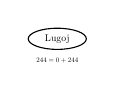
\begin{tikzpicture}[scale = 0.3]
            \node [normal] (L) {Lugoj};

            \node [length, below = 0.2em of L] (dL) {$244 = 0 + 244$};
        \end{tikzpicture}
    }

    \subfigure
    {
        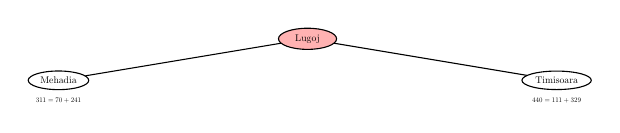
\begin{tikzpicture}[scale = 0.3]
            \node [expand] (L) {Lugoj}
                child {node [normal] (M) {Mehadia}}
                child {node [normal] (T) {Timisoara}};

            \node [length, below = 0.2em of M] (dM) {$311 = 70 + 241$};
            \node [length, below = 0.2em of T] (dT) {$440 = 111 + 329$};
        \end{tikzpicture}
    }

    \subfigure
    {
        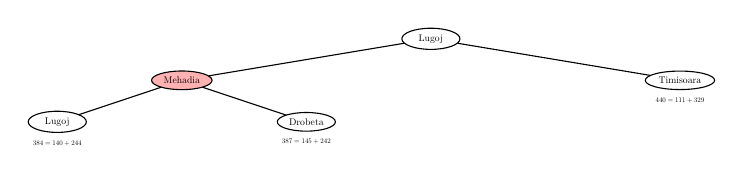
\begin{tikzpicture}[scale = 0.3]
            \node [normal] (L) {Lugoj}
                child {node [expand] (M) {Mehadia}
                    child {node [normal] (L2) {Lugoj}}
                    child {node [normal] (D) {Drobeta}}
                }
                child {node [normal] (T) {Timisoara}};

            \node [length, below = 0.2em of L2] (dL) {$384 = 140 + 244$};
            \node [length, below = 0.2em of D] (dD) {$387 = 145 + 242$};
            \node [length, below = 0.2em of T] (dT) {$440 = 111 + 329$};
        \end{tikzpicture}
    }

    \subfigure
    {
        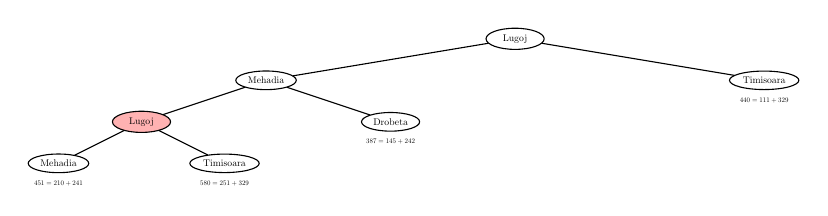
\begin{tikzpicture}[scale = 0.3]
            \node [normal] (L) {Lugoj}
                child {node [normal] (M) {Mehadia}
                    child {node [expand] (L2) {Lugoj}
                        child {node [normal] (M2) {Mehadia}}
                        child {node [normal] (T2) {Timisoara}}
                    }
                    child {node [normal] (D) {Drobeta}}
                }
                child {node [normal] (T) {Timisoara}};

            \node [length, below = 0.2em of M2] (dM2) {$451 = 210 + 241$};
            \node [length, below = 0.2em of T2] (dT2) {$580 = 251 + 329$};
            \node [length, below = 0.2em of D] (dD) {$387 = 145 + 242$};
            \node [length, below = 0.2em of T] (dT) {$440 = 111 + 329$};
        \end{tikzpicture}
    }

    \subfigure
    {
        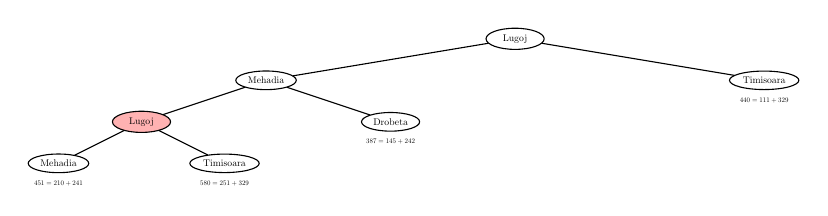
\begin{tikzpicture}[scale = 0.3]
            \node [normal] (L) {Lugoj}
                child {node [normal] (M) {Mehadia}
                    child {node [expand] (L2) {Lugoj}
                        child {node [normal] (M2) {Mehadia}}
                        child {node [normal] (T2) {Timisoara}}
                    }
                    child {node [normal] (D) {Drobeta}}
                }
                child {node [normal] (T) {Timisoara}};

            \node [length, below = 0.2em of M2] (dM2) {$451 = 210 + 241$};
            \node [length, below = 0.2em of T2] (dT2) {$580 = 251 + 329$};
            \node [length, below = 0.2em of D] (dD) {$387 = 145 + 242$};
            \node [length, below = 0.2em of T] (dT) {$440 = 111 + 329$};
        \end{tikzpicture}
    }

    \centering
    \subfigure
    {
        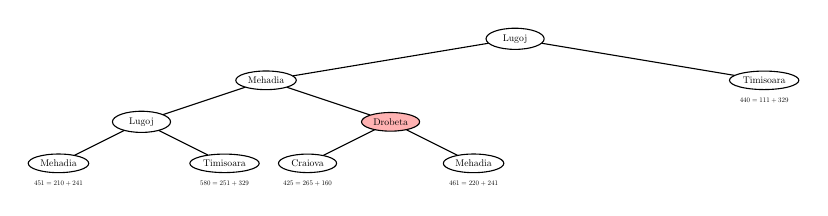
\begin{tikzpicture}[scale = 0.3]
            \node [normal] (L) {Lugoj}
                child {node [normal] (M) {Mehadia}
                    child {node [normal] (L2) {Lugoj}
                        child {node [normal] (M2) {Mehadia}}
                        child {node [normal] (T2) {Timisoara}}
                    }
                    child {node [expand] (D) {Drobeta}
                        child {node [normal] (C) {Craiova}}
                        child {node [normal] (M3) {Mehadia}}
                    }
                }
                child {node [normal] (T) {Timisoara}};

            \node [length, below = 0.2em of M2] (dM2) {$451 = 210 + 241$};
            \node [length, below = 0.2em of T2] (dT2) {$580 = 251 + 329$};
            \node [length, below = 0.2em of M3] (dM3) {$461 = 220 + 241$};
            \node [length, below = 0.2em of C] (dC) {$425 = 265 + 160$};
            \node [length, below = 0.2em of T] (dT) {$440 = 111 + 329$};
        \end{tikzpicture}
    }

    \subfigure
    {
        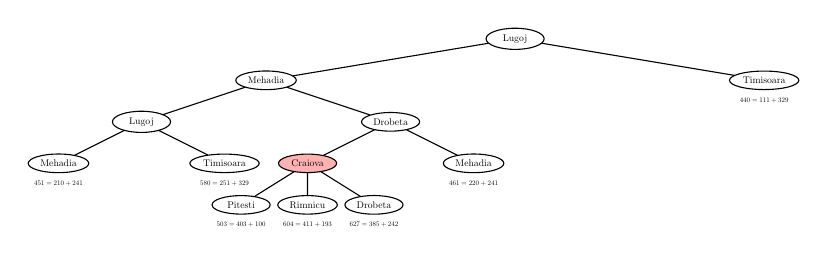
\begin{tikzpicture}[scale = 0.3]
            \node [normal] (L) {Lugoj}
                child {node [normal] (M) {Mehadia}
                    child {node [normal] (L2) {Lugoj}
                        child {node [normal] (M2) {Mehadia}}
                        child {node [normal] (T2) {Timisoara}}
                    }
                    child {node [normal] (D) {Drobeta}
                        child {node [expand] (C) {Craiova}
                            child {node [normal] (P) {Pitesti}}
                            child {node [normal] (R) {Rimnicu}}
                            child {node [normal] (D2) {Drobeta}}
                        }
                        child {node [normal] (M3) {Mehadia}}
                    }
                }
                child {node [normal] (T) {Timisoara}};

            \node [length, below = 0.2em of M2] (dM2) {$451 = 210 + 241$};
            \node [length, below = 0.2em of T2] (dT2) {$580 = 251 + 329$};
            \node [length, below = 0.2em of M3] (dM3) {$461 = 220 + 241$};
            \node [length, below = 0.2em of P] (dP) {$503 = 403 + 100$};
            \node [length, below = 0.2em of R] (dR) {$604 = 411 + 193$};
            \node [length, below = 0.2em of D2] (dD2) {$627 = 385 + 242$};
            \node [length, below = 0.2em of T] (dT) {$440 = 111 + 329$};
        \end{tikzpicture}
    }

    \subfigure
    {
        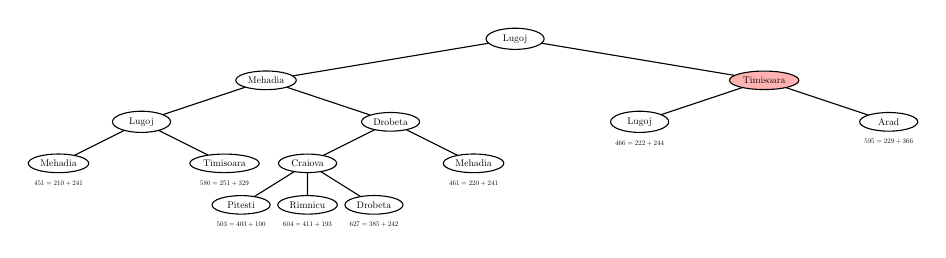
\begin{tikzpicture}[scale = 0.3]
            \node [normal] (L) {Lugoj}
                child {node [normal] (M) {Mehadia}
                    child {node [normal] (L2) {Lugoj}
                        child {node [normal] (M2) {Mehadia}}
                        child {node [normal] (T2) {Timisoara}}
                    }
                    child {node [normal] (D) {Drobeta}
                        child {node [normal] (C) {Craiova}
                            child {node [normal] (P) {Pitesti}}
                            child {node [normal] (R) {Rimnicu}}
                            child {node [normal] (D2) {Drobeta}}
                        }
                        child {node [normal] (M3) {Mehadia}}
                    }
                }
                child {node [expand] (T) {Timisoara}
                    child {node [normal] (L3) {Lugoj}}
                    child {node [normal] (A) {Arad}}
                };

            \node [length, below = 0.2em of M2] (dM2) {$451 = 210 + 241$};
            \node [length, below = 0.2em of T2] (dT2) {$580 = 251 + 329$};
            \node [length, below = 0.2em of M3] (dM3) {$461 = 220 + 241$};
            \node [length, below = 0.2em of P] (dP) {$503 = 403 + 100$};
            \node [length, below = 0.2em of R] (dR) {$604 = 411 + 193$};
            \node [length, below = 0.2em of D2] (dD2) {$627 = 385 + 242$};
            \node [length, below = 0.2em of L3] (dL3) {$466 = 222 + 244$};
            \node [length, below = 0.2em of A] (dA) {$595 = 229 + 366$};
        \end{tikzpicture}
    }
\end{figure}

\begin{figure}[t]
    \centering
    \subfigure
    {
        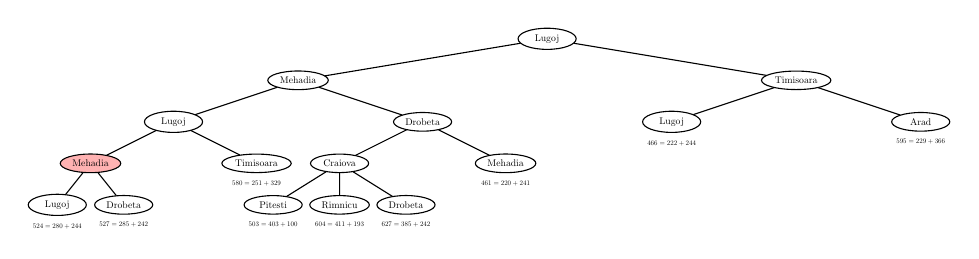
\begin{tikzpicture}[scale = 0.3]
            \node [normal] (L) {Lugoj}
                child {node [normal] (M) {Mehadia}
                    child {node [normal] (L2) {Lugoj}
                        child {node [expand] (M2) {Mehadia}
                            child {node [normal] (L4) {Lugoj}}
                            child {node [normal] (D3) {Drobeta}}
                        }
                        child {node [normal] (T2) {Timisoara}}
                    }
                    child {node [normal] (D) {Drobeta}
                        child {node [normal] (C) {Craiova}
                            child {node [normal] (P) {Pitesti}}
                            child {node [normal] (R) {Rimnicu}}
                            child {node [normal] (D2) {Drobeta}}
                        }
                        child {node [normal] (M3) {Mehadia}}
                    }
                }
                child {node [normal] (T) {Timisoara}
                    child {node [normal] (L3) {Lugoj}}
                    child {node [normal] (A) {Arad}}
                };

            \node [length, below = 0.2em of L4] (dL4) {$524 = 280 + 244$};
            \node [length, below = 0.2em of D3] (dD3) {$527 = 285 + 242$};
            \node [length, below = 0.2em of T2] (dT2) {$580 = 251 + 329$};
            \node [length, below = 0.2em of M3] (dM3) {$461 = 220 + 241$};
            \node [length, below = 0.2em of P] (dP) {$503 = 403 + 100$};
            \node [length, below = 0.2em of R] (dR) {$604 = 411 + 193$};
            \node [length, below = 0.2em of D2] (dD2) {$627 = 385 + 242$};
            \node [length, below = 0.2em of L3] (dL3) {$466 = 222 + 244$};
            \node [length, below = 0.2em of A] (dA) {$595 = 229 + 366$};
        \end{tikzpicture}
    }

    \subfigure
    {
        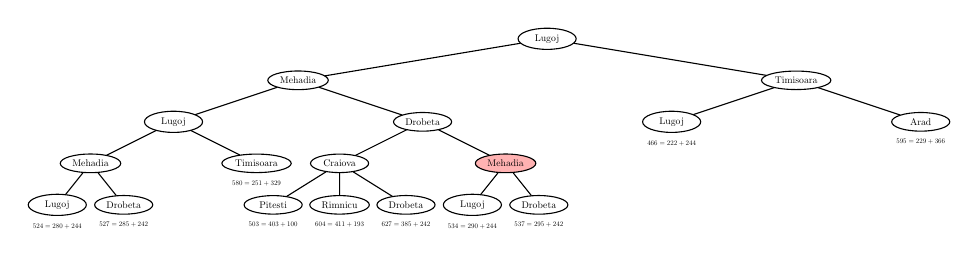
\begin{tikzpicture}[scale = 0.3]
            \node [normal] (L) {Lugoj}
                child {node [normal] (M) {Mehadia}
                    child {node [normal] (L2) {Lugoj}
                        child {node [normal] (M2) {Mehadia}
                            child {node [normal] (L4) {Lugoj}}
                            child {node [normal] (D3) {Drobeta}}
                        }
                        child {node [normal] (T2) {Timisoara}}
                    }
                    child {node [normal] (D) {Drobeta}
                        child {node [normal] (C) {Craiova}
                            child {node [normal] (P) {Pitesti}}
                            child {node [normal] (R) {Rimnicu}}
                            child {node [normal] (D2) {Drobeta}}
                        }
                        child {node [expand] (M3) {Mehadia}
                            child {node [normal] (L5) {Lugoj}}
                            child {node [normal] (D4) {Drobeta}}
                        }
                    }
                }
                child {node [normal] (T) {Timisoara}
                    child {node [normal] (L3) {Lugoj}}
                    child {node [normal] (A) {Arad}}
                };

            \node [length, below = 0.2em of L4] (dL4) {$524 = 280 + 244$};
            \node [length, below = 0.2em of D3] (dD3) {$527 = 285 + 242$};
            \node [length, below = 0.2em of T2] (dT2) {$580 = 251 + 329$};
            \node [length, below = 0.2em of L5] (dL5) {$534 = 290 + 244$};
            \node [length, below = 0.2em of D4] (dD4) {$537 = 295 + 242$};
            \node [length, below = 0.2em of P] (dP) {$503 = 403 + 100$};
            \node [length, below = 0.2em of R] (dR) {$604 = 411 + 193$};
            \node [length, below = 0.2em of D2] (dD2) {$627 = 385 + 242$};
            \node [length, below = 0.2em of L3] (dL3) {$466 = 222 + 244$};
            \node [length, below = 0.2em of A] (dA) {$595 = 229 + 366$};
        \end{tikzpicture}
    }

    \subfigure
    {
        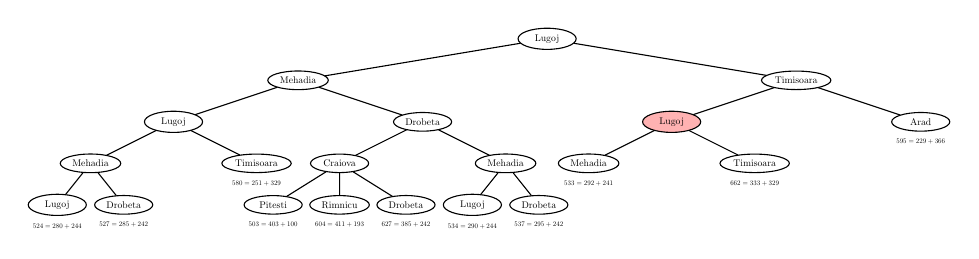
\begin{tikzpicture}[scale = 0.3]
            \node [normal] (L) {Lugoj}
                child {node [normal] (M) {Mehadia}
                    child {node [normal] (L2) {Lugoj}
                        child {node [normal] (M2) {Mehadia}
                            child {node [normal] (L4) {Lugoj}}
                            child {node [normal] (D3) {Drobeta}}
                        }
                        child {node [normal] (T2) {Timisoara}}
                    }
                    child {node [normal] (D) {Drobeta}
                        child {node [normal] (C) {Craiova}
                            child {node [normal] (P) {Pitesti}}
                            child {node [normal] (R) {Rimnicu}}
                            child {node [normal] (D2) {Drobeta}}
                        }
                        child {node [normal] (M3) {Mehadia}
                            child {node [normal] (L5) {Lugoj}}
                            child {node [normal] (D4) {Drobeta}}
                        }
                    }
                }
                child {node [normal] (T) {Timisoara}
                    child {node [expand] (L3) {Lugoj}
                        child {node [normal] (M4) {Mehadia}}
                        child {node [normal] (T3) {Timisoara}}
                    }
                    child {node [normal] (A) {Arad}}
                };

            \node [length, below = 0.2em of L4] (dL4) {$524 = 280 + 244$};
            \node [length, below = 0.2em of D3] (dD3) {$527 = 285 + 242$};
            \node [length, below = 0.2em of T2] (dT2) {$580 = 251 + 329$};
            \node [length, below = 0.2em of L5] (dL5) {$534 = 290 + 244$};
            \node [length, below = 0.2em of D4] (dD4) {$537 = 295 + 242$};
            \node [length, below = 0.2em of P] (dP) {$503 = 403 + 100$};
            \node [length, below = 0.2em of R] (dR) {$604 = 411 + 193$};
            \node [length, below = 0.2em of D2] (dD2) {$627 = 385 + 242$};
            \node [length, below = 0.2em of M4] (dM4) {$533 = 292 + 241$};
            \node [length, below = 0.2em of T3] (dT3) {$662 = 333 + 329$};
            \node [length, below = 0.2em of A] (dA) {$595 = 229 + 366$};
        \end{tikzpicture}
    }

    \subfigure
    {
        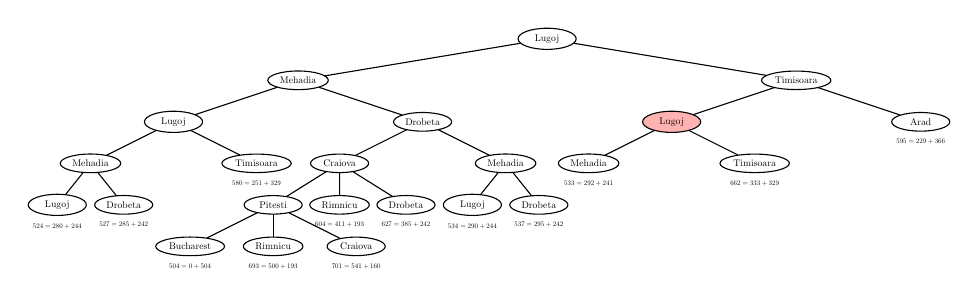
\begin{tikzpicture}[scale = 0.3]
            \node [normal] (L) {Lugoj}
                child {node [normal] (M) {Mehadia}
                    child {node [normal] (L2) {Lugoj}
                        child {node [normal] (M2) {Mehadia}
                            child {node [normal] (L4) {Lugoj}}
                            child {node [normal] (D3) {Drobeta}}
                        }
                        child {node [normal] (T2) {Timisoara}}
                    }
                    child {node [normal] (D) {Drobeta}
                        child {node [normal] (C) {Craiova}
                            child {node [normal] (P) {Pitesti}
                                child {node [normal] (B) {Bucharest}}
                                child {node [normal] (R2) {Rimnicu}}
                                child {node [normal] (C2) {Craiova}}
                            }
                            child {node [normal] (R) {Rimnicu}}
                            child {node [normal] (D2) {Drobeta}}
                        }
                        child {node [normal] (M3) {Mehadia}
                            child {node [normal] (L5) {Lugoj}}
                            child {node [normal] (D4) {Drobeta}}
                        }
                    }
                }
                child {node [normal] (T) {Timisoara}
                    child {node [expand] (L3) {Lugoj}
                        child {node [normal] (M4) {Mehadia}}
                        child {node [normal] (T3) {Timisoara}}
                    }
                    child {node [normal] (A) {Arad}}
                };

            \node [length, below = 0.2em of L4] (dL4) {$524 = 280 + 244$};
            \node [length, below = 0.2em of D3] (dD3) {$527 = 285 + 242$};
            \node [length, below = 0.2em of T2] (dT2) {$580 = 251 + 329$};
            \node [length, below = 0.2em of L5] (dL5) {$534 = 290 + 244$};
            \node [length, below = 0.2em of D4] (dD4) {$537 = 295 + 242$};
            \node [length, below = 0.2em of B] (dB) {$504 = 0 + 504$};
            \node [length, below = 0.2em of R2] (dR2) {$693 = 500 + 193$};
            \node [length, below = 0.2em of C2] (dC2) {$701 = 541 + 160$};
            \node [length, below = 0.2em of R] (dR) {$604 = 411 + 193$};
            \node [length, below = 0.2em of D2] (dD2) {$627 = 385 + 242$};
            \node [length, below = 0.2em of M4] (dM4) {$533 = 292 + 241$};
            \node [length, below = 0.2em of T3] (dT3) {$662 = 333 + 329$};
            \node [length, below = 0.2em of A] (dA) {$595 = 229 + 366$};
        \end{tikzpicture}
    }
    \caption{使用A$^*$搜索应用直线距离启发式求解从 Lugoj 到 Bucharest 问题}
    \label{figure:1}
\end{figure}



\end{document}